\documentclass[12pt,a4paper,oneside]{report}
\usepackage{amsthm}
\usepackage{amsmath}
\usepackage{tikz}
\usetikzlibrary{shapes,arrows,automata,trees, shadows,decorations.pathmorphing}
\begin{document}
\title{CS375 Week 6}
\author{Jason N Mansfield}
\maketitle
\section{}

$$L =\{a^n b^{2n}\mid n \ge 1\} = \{abb, aabbbb, aaabbbbbb,...\}$$



\begin{proof}
For any regular language L, there exists a number p such that for any string w in L of length at least p there are strings x,y,z such that
\begin{itemize}
\item $w =  xyz$
\item $\mid xy \mid \le  p$
\item $\mid y \mid \ge 1$
\item Then $x = a^n, y = a^n, z = b^{p+1}$
\item $xy^2z \ni L$
\item This is a contradiction so language is nonregular.
\end{itemize}
\end{proof}

\begin{figure}
\begin{center}
\caption{Pumping Lemma Contradiction}
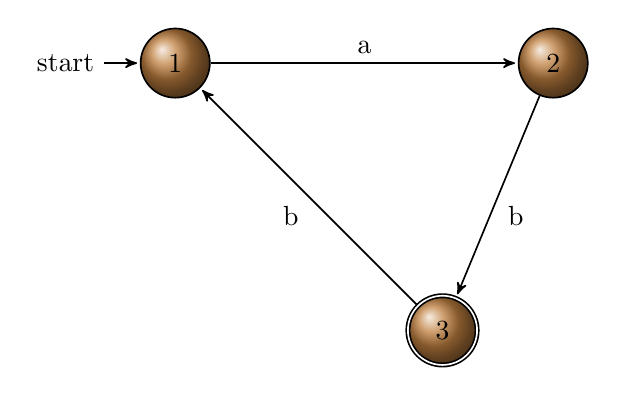
\begin{tikzpicture}[->,>=stealth',shorten >=1pt,auto,node distance=4.8cm, semithick]
\tikzstyle{every state}=[draw=black,text=black, ball color=brown]
\node[initial,state] (1) {1};
\node[state][right of=1](2){2};
\node[state, accepting][below right of=1](3){3};
\path (1)edge node{a}(2)
          (2)edge node{b}(3)
          (3)edge node{b}(1);       
\end{tikzpicture} 
\end{center}
\end{figure}
\section{}
\begin{enumerate}
\item Palindromes
\begin{enumerate}
\item If w = xyz.
\item And if x = a, y = b, z = a.
\item or if x = b, y = a, z = b.
\item Then $w = a^{90 + 1}ba^{90}$
\item and $w = b^{90 + 1}ab^{90}$
\item Therefore Palindromes are nonregular
\end{enumerate}
\item Equal
\begin{enumerate}
\item
\end{enumerate}
\end{enumerate}
\section{}

\end{document}